% \documentclass[12pt]{article}

% preamble

\documentclass[12pt]{article}

% preamble

% TO DOUBLESPACE THE PRINTOUT, INSERT THE COMMAND
% \renewcommand{\baselinestretch}{2}

%\setlength{\textheight}{8.5in}
%\setlength{\textwidth}{6.25in}
%\setlength{\topmargin}{0.0in}

\newtheorem{defn}{Definition}
\newtheorem{cor}[defn]{Corollary}
\newtheorem{lemma}[defn]{Lemma}
\newtheorem{obs}[defn]{Observation}
\newtheorem{prop}[defn]{Proposition}
\newtheorem{thm}[defn]{Theorem}
\newtheorem{cond}[defn]{Condition}
\newtheorem{conj}[defn]{Conjecture}
\newtheorem{ass}[defn]{Assumption}
\newtheorem{example}[defn]{Example}
\newtheorem{rem}[defn]{Remark}

\newcommand{\abs}[1]{\left| #1 \right| }
\newcommand{\ans}{\noi\textbf{Answer: }}
\newcommand{\ds}{\displaystyle}
\newcommand{\dydx}{\ds \frac{dy}{dx}}
\newcommand{\infnorm}[1]{\ensuremath{\left\| #1 \right\|_{\infty}}}
\newcommand{\ital}{\textit}
\newcommand{\la}{\langle}
\newcommand{\lb}{\left\{}
\newcommand{\lp}{\left(}
\newcommand{\N}{I\!\!N}
\newcommand{\noi}{\noindent}
\newcommand{\norm}[1]{\ensuremath{\left\| #1 \right\| }}
\newcommand{\oon}{\frac{1}{n}}
\newcommand{\pic}[1]{\begin{center}\includegraphics{#1}\end{center}}
\newcommand{\R}{I\!\!R}
\newcommand{\ra}{\rangle}
\newcommand{\rb}{\right\}}
\newcommand{\rp}{\right)}
\newcommand{\skp}{\vspace{\baselineskip}}
\newcommand{\snsp}{@!@!@!@!@!}
\newcommand{\trm}{\textrm}
\newcommand{\ve}{\ensuremath{\varepsilon}}

% document

\usepackage{amsmath}
\usepackage{graphicx} 
\usepackage{hyperref}
\usepackage{soul}
\usepackage{xcolor}

% document

\begin{document}

\section*{Mom and Erd\"{o}s \\
\begin{small} \begin{color}{gray} (January 29, 2025) \end{color} \end{small}}


My Mom got a Master's Degree in Mathematics in the early 90's. At some point in her coursework one of her professors shared a problem that I think was a sort of extra credit exercise, and Mom shared it with me. I was teaching math at a summer program at Boston College at the time, and I spent an evening or two a week staffing a little-used tutoring desk in a lounge in one of the dorms in which the camp participants stayed. I spent one such evening solving this problem and realized that the childish pride in impressing one's mother never quite goes away. The problem is to prove Theorem \ref{Erdos}, and I discovered later on that it was posed in the problems section of the \textit{American Mathematical Monthly} by Paul Erd\"{o}s in 1993 \cite{ERDOS}.

\begin{thm} \label{Erdos} Let $\ds A,B$, and $C$ be the vertices of a triangle inscribed in a unit circle, and let $P$ be a point in the interior of the triangle $ABC$. Then
\begin{equation} \label{statement}
  \abs{PA}\cdot \abs{PB}\cdot \abs{PC}<\frac{32}{27}.
\end{equation}
\end{thm}

Thinking of the vertices as complex numbers, for any point $Z$ in the triangle, the distance product in (\ref{statement}) is the modulus of the cubic polynomial $\ds \abs{ (Z-A)(Z-B)(Z-C)}$. The Maximum Modulus Principle from complex analysis guarantees that the maximum modulus of this polynomial occurs on the boundary of the triangle, so if the inequality can be proved for points on the boundary, it will be enough. 

Figure \ref{image2} is useful to illustrate the following argument. Suppose $Z$ is on side $AB$, and let $E$ be the midpoint of this side. Then $\ds AE = EB$, and $\ds AO = OB = 1$ because they are both radii of the unit circle. This last fact means that triangle $\ds AOB$ is isoceles, and so $\ds \angle OAE = \angle OBE$, and now the triangles are congruent via side-angle-side. Since the angles $\ds OEA$ and $\ds OEB$ are equal and supplementary, they must each be right angles and so the triangles $\ds OAE$ and $\ds OBE$ are right triangles.

By Lemma \ref{lemma}, to maximize $\ds \abs{ (Z-A)(Z-B)(Z-C)}$, we should choose $C$ to be collinear with $Z$ and the center of the circle $O$, so
\[
  \abs{OE} = \sqrt{1-\abs{AE}^2} = \sqrt{1 - (\abs{AB}/2)^2} = \sqrt{1-\abs{AB}^2/4}
\]
and
\begin{align*}
 \abs{ZO} &= \sqrt{\abs{OE}^2 + \abs{ZE}^2} \\
 &= \sqrt{1-\abs{AB}^2/4 + (\abs{AZ} - \abs{AE})^2} \\
 &=  \sqrt{1-\abs{AB}^2/4 + (\abs{AZ} - \abs{AB}/2)^2} \\
 &= \sqrt{1-\abs{AZ}\abs{BZ}}
\end{align*}

Letting $\ds x = \abs{AZ}\abs{BZ}$, 
\begin{align*}
  \abs{AZ}\cdot \abs{BZ}\cdot\abs{CZ} &= x (1+\abs{ZO}) \\
  &= x\lp 1+\sqrt{1-x} \rp
\end{align*}

$\ds x$ is the product of positive numbers whose sum is not more than 2, so $\ds x\in [0,1]$. The maximum of $\ds x\lp 1+\sqrt{1-x} \rp$ on $\ds [0,1]$ occurs at $\ds x = \frac{8}{9}$, and 
\[
  \lp \frac{8}{9} \rp \lp 1+\sqrt{1-\lp \frac{8}{9} \rp} \rp = \frac{32}{27}
\]

\begin{lemma} \label{lemma} Let $Z$ be a point inside a circle with center $O$. The point $D$ on the circle that maximizes $\overline{Z D}$ is collinear with $Z$ and $O$.
\end{lemma}

\begin{proof} Let $C$ be any point on the circle, and let $D$ be the point on the circle that is collinear with $O$ and $Z$ such that $\ds \overline{ZD}$ is larger than the radius of the circle. Let $X$ be the perpendicular foot from $O$ to $ZC$. Then
\begin{eqnarray*}
 \abs{ZC} & = & \abs{ZX} + \abs{XC} \\
 & \leq & \abs{ZO} + \abs{OC} \\
 & = & \abs{ZO} + \abs{OD} \\
 & = & \abs{ZD}
\end{eqnarray*}

\begin{figure}[h]
\centering
\caption{Illustration of Lemma \ref{lemma}}
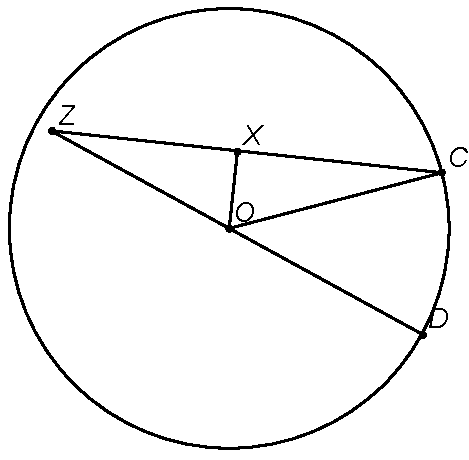
\includegraphics{images/image1}
\end{figure}
\end{proof}

\begin{figure}[h]
\centering
\caption{Illustration of Theorem \ref{Erdos}}
\label{image2}
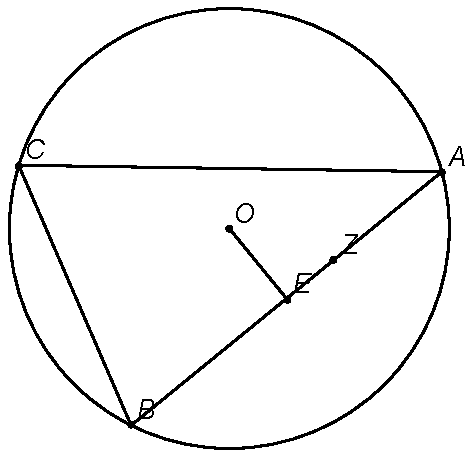
\includegraphics{images/image2}
\end{figure}

\begin{thebibliography}{99}

\bibitem{ERDOS} Erd\"{o}s, Paul, et al. ``Problems: 10282-10289." \textit{The American Mathematical Monthly}, vol. 100, no. 2, 1993, pp. 184–85. JSTOR, \url{https://doi.org/10.2307/2323782}.

\end{thebibliography}


\end{document}
